\chapter{Profils}
\begin{figure}[hlc]
	\center

	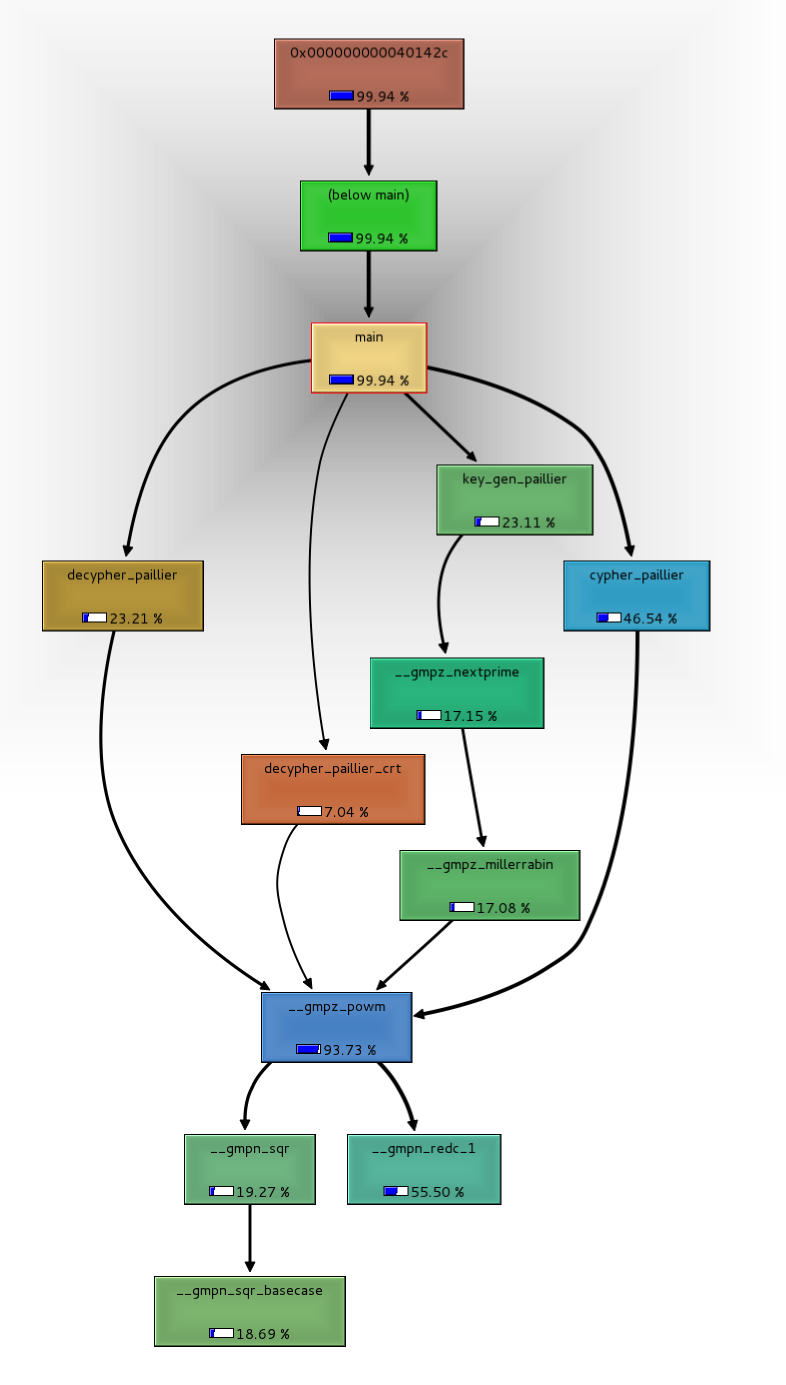
\includegraphics[height=0.8\textheight]{proff.eps}
	
	\caption{Profil montrant l'utilisation des ressources par les différentes méthodes implantées.} 
\end{figure}

Le profil a été réalisé sur le code suivant:
\begin{lstlisting}[language=C,emph={},caption=Code du test de profil., label=code:profil]
#include <stdio.h>
#include "paillier.h"
int main(){
	pvt_key pvt;
	public_key pub;
	mpz_t message, encripted, message_prime, tmp;
	int i;
	_rnd_paillier= NULL;

	mpz_init(message);
	mpz_init(message_prime);
	mpz_init(encripted);
	mpz_init(tmp);

	pvt = key_gen_paillier(1024LU);
	pub = get_public_paillier(pvt);

	for(i = 0;i<10;i++){
		checkRandomInit();
		mpz_urandomm(message, *_rnd_paillier, pub->n);
		cypher_paillier(encripted,message,pub);
		decypher_paillier(message_prime,encripted,pvt);
		decypher_paillier_crt(message_prime,tmp,encripted,pvt);
	}
	cleankeys(&pvt,NULL);
	cleankeys(NULL,&pub);
	return 0;
}
\end{lstlisting}
